
\documentclass[ms.tex]{subfiles}
\begin{document}

\section{Introduction}
\label{sec:intro}

From a nucleosynthesis perspective, nitrogen (N) is a unique element.
Along with carbon (C) and helium (He), it is one of only three elements lighter
than iron peak nuclei who owe a significant portion of their abundances to
asymptotic giant branch (AGB) stars~\citep{Johnson2019}.
N is also a by-product of the nuclear fusion reactions converting hydrogen (H)
into He in stars more massive than the sun with nonzero metallicity.
The CNO cycle\footnote{
	\Ctwelve(p, $\gamma$)\Nthirteen($\beta^+$ $\nu_e$)\Cthirteen(p, $\gamma$)
	\Nfourteen(p, $\gamma$)\Ofifteen($\beta^+$ $\nu_e$)\Nfifteen(p, $\alpha$)
	\Ctwelve
} catalyses the proton-proton chain of nuclear reactions
\citep*[e.g.][]{Suliga2020} using C, N, and oxygen (O) target nuclei.
The slowest component of this chain reaction by far is the
\Nfourteen(p,$\gamma$)\Ofifteen~component.
As a consequence of this bottleneck, to first order the effect of the CNO cycle
is to convert all of the C and O isotopes present in a star's core into
\Nfourteen.
Furthermore, N is among a select group of elements whose observed abundances
in stellar spectra often do not reflect the star's birth abundances.
Because N is produced in main sequence stars via the CNO cycle, its abundances
in a star's core become enhanced relative to what the star was born with.
Upon becoming a red giant, internal mixing processes (i.e. dredge-up) bring this
N-enhanced material to the photosphere.
This phenomenon is both expected from theoretical models and observed in open
and globular clusters~\citep{Gilroy1989, Korn2007, Lind2008, Souto2018,
Souto2019, Vincenzo2021}.

\begin{figure*}
\centering
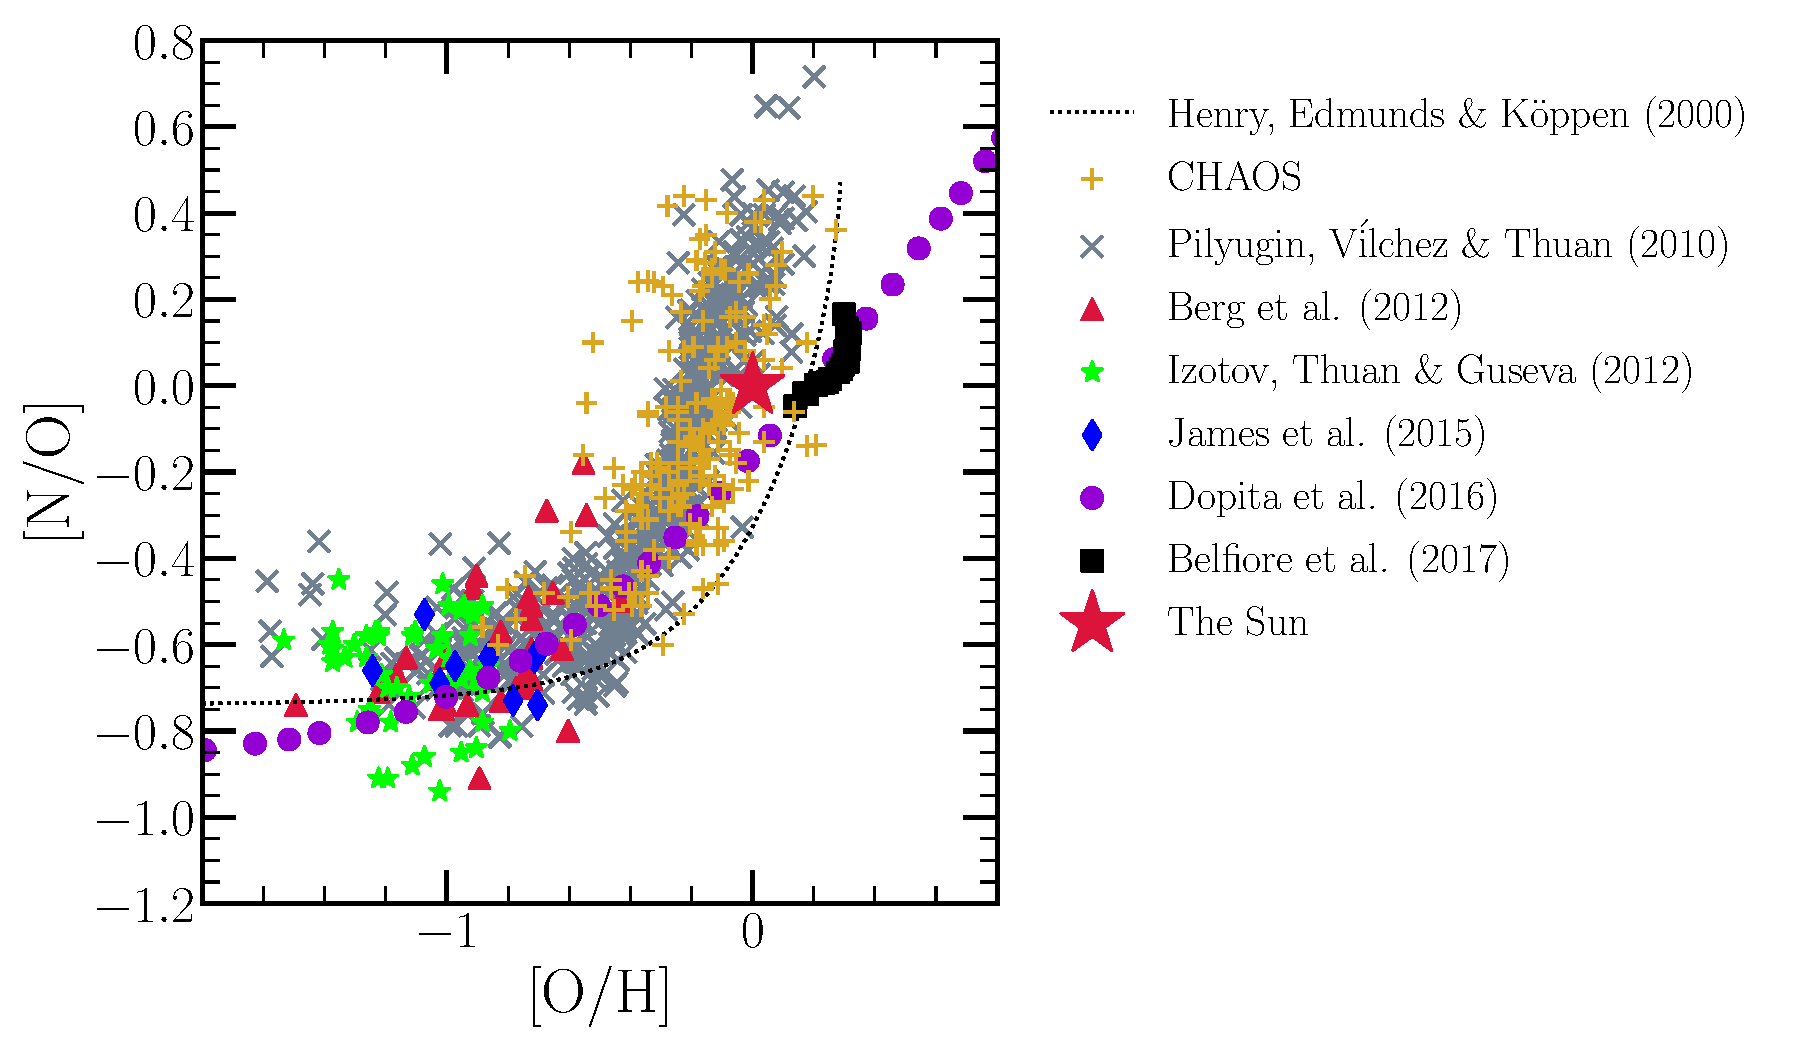
\includegraphics[scale = 0.63]{no_oh_observed.pdf}
\caption{
	The~\ohno~relation as observed in different galactic environments:
	HII regions from the first six CHAOS galaxies (golden +'s: NGC 3184, NGC
	628, NGC 5194, NGC 5457, M101, and NGC 2403;~\citealp{Berg2020,
	Skillman2020, Rogers2021}) and other nearby NGC spiral galaxies (grey X's;
	\citealp{Pilyugin2010}), HII regions in blue diffuse star forming dwarf
	galaxies (red triangles:~\citealp{Berg2012}; green stars:
	\citealp{Izotov2012}; blue diamonds:~\citealp{James2015}), in local stars
	and HII regions (purple circles:~\citealp{Dopita2016}), and in the MaNGA
	IFU survey (black squares:~\citealp{Belfiore2017}).
	The fit to~\no~as a function of~\oh~in Galactic and extragalactic HII
	regions by~\citet{Henry2000} is shown in a black dotted line.
	We omit all uncertainties for visual clarity.
	The Sun, at (0, 0) on this plot by definition, is marked by a large red
	star. 
}
\label{fig:no_oh_observed}
\end{figure*}

Both observationally and theoretically, N is among the more well-studied
elements.
Of particular interest in this paper is the correlation between the abundances
of N and O, usually observed in the gas phase.
In Fig.~\ref{fig:no_oh_observed}, we present a compilation of such measurements:
\begin{enumerate}
	\item[\textbf{1.}] HII regions in the first six CHAOS\footnote{
		CHAOS: CHemical Abundances Of Spirals~\citep{Berg2015}
	} galaxies (NGC 3184, NGC 628, NGC 5194, NGC 5457, M101, NGC 2403;
	\citealp{Berg2020, Skillman2020, Rogers2021}).

	\item[\textbf{2.}] HII regions in nearby NGC spirals~\citep*{Pilyugin2010}.

	\item[\textbf{3.}] HII regions in blue, diffuse star forming dwarf galaxies
	(\citealp{Berg2012};~\citealp*{Izotov2012};~\citealp{James2015}).

	\item[\textbf{4.}] Local stars and HII regions~\citep{Dopita2016}.

	\item[\textbf{5.}] Galactic and extragalactic HII regions
	\citep*{Henry2000}.

	\item[\textbf{6.}] Star-forming regions in 550  nearby galaxies in the
	MaNGA IFU\footnote{
		MaNGA: Mapping Nearby Galaxies at Apache Point Observatory
		\citep{Bundy2015}.
		IFU: Integral Field Unit.
	} survey~\citep{Belfiore2017}.
\end{enumerate}
Despite intrinsic scatter and some systematic variation in how the abundances
are determined, this~\ohno\footnote{
	We follow standard notation where [X/Y]
	$\equiv \log_{10}(X/Y) - \log_{10}(X/Y)_\odot$.
} relation is more or less the same across a wide range of astrophysical
environments.
Furthermore, recent arguments from both theoretical~\citep{Vincenzo2018} and
observational perspectives~\citep{HaydenPawson2021} suggest that this relation
is largely redshift-invariant.
Previous studies have interpreted this universality as an indication that the
relation is nucleosynthetic in origin, reflecting the differences between
``primary'' and ``secondary'' N production whereby the primary yields do not
depend on the initial metal content of a star but the secondary yields do
(\citealp{VilaCostas1993};~\citealp*{vanZee1998};~\citealp{Henry1999,
PerezMontero2009, Berg2012};~\citealp*{Pilyugin2012};~\citealp{Andrews2013}).
Here we are interested in the origin of both the shape and scatter in this
trend using the Milky Way as a case test.
\par
N is not unique in that perhaps the largest source of uncertainty in
understanding its abundances is that accurate and precise nucleosynthetic yields
from various enrichment channels remain elusive.
Presently, no combination of models for nucleosynthesis in and explosions of
massive stars is able to reproduce the observed abundance pattern of the
elements, and N is no exception~\citep{Griffith2021a}.
Recently,~\citet*{Grisoni2021} argued that rotating massive stars play a key
role in establishing the N abundances seen in metal-poor stars in the Milky Way.
Rotation has a considerable impact on the N yields of massive stars, because the
internal mixing that it causes~\citep{Zahn1992, Maeder1998, Lagarde2012} brings
internally produced C and O nuclei into the H-burning shell where they can be
processed into~\Nfourteen~via the CNO cycle~\citep{Heger2010, Frischknecht2016,
Andrews2017}.
We find similar results here comparing various theoretical models for
massive star nucleosynthesis (see discussion in~\S~\ref{sec:yields:ccsne}).
\par
Theoretical models for AGB star nucleosynthesis predict N yields to vary as a
function of progenitor mass and metallicity~\citep{Cristallo2011, Cristallo2015,
Karakas2010, Karakas2016, Karakas2018, Ventura2013, Ventura2014, Ventura2018,
Ventura2020}.
In sufficiently massive AGB stars, the base of the convective envelope is hot
enough to activate proton capture reactions, allowing the CNO cycle to convert
C and O isotopes in~\Nfourteen: a process known as hot bottom burning.
AGB stars are also known to experience thermal pulsations, and often these
pulations are accompanied by a penetration of the convective enevelope into the
CO-rich core, bringing some of this material into the envelope: a process known
as third dredge-up.\footnote{
	Here the time adverbial ``third'' refers only to the fact that these
	dredge-up episodes are occurring while the star is on the asymptotic giant
	branch. Because they are associated with the thermal pulsations of AGB
	stars, there are many episodes of third dredge-up.
}
When both processes are active, third-dredge up adds new seed nuclei for hot
bottom burning to turn into~\Nfourteen, substantially increasing the N yields.
We demonstrate in~\S\S~\ref{sec:yields:agb} and~\ref{sec:yields:imf_agb} that
various theoretical models predict significantly different N yields for high
mass AGB stars as a consequence of how third dredge-up and hot bottom burning
occur in the models.
The differences in these processes are in turn a consequence of the
microphysical assumptions built into the stellar evolution models (e.g. mass
loss, opacity, convection and convective boundaries, nuclear reaction networks).
\par
In this paper, we aim to constrain N yields empirically by testing the
performance of various ``off-the-shelf'' yield models within the framework of
galactic chemical evolution (GCE) models.
To this end we use the multi-zone model for the Milky Way published in
\citet{Johnson2021}, which treats the Galaxy as a series of concentric rings,
describing each ring as a conventional one-zone model of chemical evolution
(see discussion in~\S~\ref{sec:multizone}).
This approach has been employed in the past to compute abundance simultaneously
for many Galactic regions (\citealp{Matteucci1989, Wyse1989, Prantzos1995,
Schoenrich2009};~\citealp*{Minchev2013, Minchev2014};~\citealp{Minchev2017};
\citealp*{Sharma2021}).
In this paper, we assess what is required of N yields in order to reproduce
various observed results, in particular the gas-phase~\ohno~relation
illustrated in Fig.~\ref{fig:no_oh_observed}.
Since a number of previous studies argue this result is nucleosynthetic in
origin~\citep[e.g.][]{Pilyugin2012, Andrews2013}, our results from a GCE model
for the Milky Way should apply to other systems as well.
\par
In a sample of 6,507 galaxies from the MaNGA IFU survey~\citep{Bundy2015},
\citet{Schaefer2020} demonstrate that the intrinsic scatter in
the~\ohno~relation at fixed galaxy mass is correlated with variations in the
local star formation efficiency (SFE).
In regions of slower star formation,~\no~tends to be slightly higher at
fixed~\oh~(see their Fig. 4).
This is expected from simple GCE models, because more AGB stars enrich the
ISM with N by the time a given~\oh~is reached~\citep[e.g.][]{Molla2006,
Vincenzo2016a}.
However,~\citet{Schaefer2020} did not rule out stellar migration as an
additional source of scatter in the gas-phase~\ohno~relation.
In principle, there could be a deficit or surplus of N-producing AGB stars in a
given Galactic region at any time simply because the orbits are evolving,
driving additional scatter in the correlation.
The~\citet{Johnson2021} GCE model is the ideal tool with which to test this
hypothesis.
The novel difference between theirs and previous models with similar
motivations is that it allows stellar populations to enrich distributions of
radii as they migrate.
Originally developed to study the abundances of O and iron (Fe), this aspect of
Galactic evolution turned out to have an important impact on the delayed type
Ia supernova (SN Ia) enrichment of Fe, causing complex fluctuations in the
enrichment rates with time at fixed radius.
Here we use the same methodology to test for similar effects in the delayed AGB
star production of N and to assess the extent to which migration and
variability in the SFE drive scatter in the observed~\ohno~relation.
\par
By additionally making use of stellar abundance data, we can test the N
abundances predicted by our model against observables unavailable for the gas
phase, such as age and~\ofe.
Using data from the Apache Point Observatory Galaxy Evolution Experiment
(APOGEE;~\citealp{Majewski2017}),~\citet{Vincenzo2021} demonstrate that when
stellar N abundances are corrected for internal mixing processes, the
correlations with stellar age and other elemental abundances are affected.
Whether or not our GCE model is able to reproduce their corrected data
constitutes a valuable test not only of our understanding of N nucleosynthesis,
but also the accuracy of the~\citet{Vincenzo2021} measurements which take a
model-dependent approach to estimate the birth abundances of N for APOGEE disc
stars with available age measurements.


\end{document}

